\documentclass[11pt,a4paper]{article}

\usepackage[utf8]{inputenc}
\usepackage[T1]{fontenc}
\usepackage{amsmath,amssymb,amsfonts}
\usepackage{graphicx}
\usepackage{booktabs}
\usepackage{hyperref}
\usepackage[margin=1in]{geometry}
\usepackage{caption}
\usepackage{subcaption}
\usepackage{enumitem}
\usepackage{xcolor}
\usepackage[numbers]{natbib}
\bibliographystyle{unsrtnat}

\hypersetup{
    colorlinks=true,
    linkcolor=blue!60!black,
    citecolor=blue!60!black,
    urlcolor=blue!60!black,
}

\title{Interpretable Minimal Transformers: Geometry as Algorithm}
\author{}
\date{}

\begin{document}
\maketitle

\begin{abstract}
We present a framework for building and interpreting minimal transformer language models trained on procedurally generated integer sequences. By constraining the embedding dimension to $n_{\mathrm{embd}} = 2$ and the head size to $d_k = 2$, we enable full two-dimensional visualization of every internal representation---embeddings, query/key/value transforms, attention outputs, residual streams, and the language-model head's decision boundaries. Our central claim is that \textbf{the learned geometry implies an algorithm}: the arrangement of points and boundaries in $\mathbb{R}^2$ can be read as a step-by-step procedure. For the \emph{plus-last-even} task, the model encodes the \texttt{+} operator at a query position, attends to keys of the most recent even number, retrieves its value, and maps the resulting state into the correct output region via the residual connection and LM head. We introduce a suite of interpretability visualizations that make this algorithmic reading explicit, and provide training-evolution animations showing how the algorithmic geometry emerges during learning. The framework offers a pedagogical and experimental testbed where \emph{seeing the geometry is seeing the algorithm}.
\end{abstract}

%----------------------------------------------------------------------
\section{Introduction}

Understanding how transformers process sequences remains a central challenge in mechanistic interpretability. Large-scale models achieve strong performance but their internal representations are high-dimensional and opaque: one can probe attention or activations, but a \emph{complete} picture of information flow from input to output remains elusive. At the other extreme, toy models on synthetic tasks are easier to analyze but often lack the full machinery of production transformers---attention over variable context, residual connections, and a learned output head.

We bridge this gap with \textbf{minimal transformers}: models that retain the full structure of a decoder-only transformer (token and positional embeddings, single-head causal self-attention, residual connections, a feedforward layer, and an LM head) but are constrained to two-dimensional embeddings and head dimension. Every internal state---embeddings, queries, keys, values, attention outputs, residual sums, and pre-softmax logit vectors---lives in $\mathbb{R}^2$. No PCA, t-SNE, or UMAP is required; the model's geometry is directly visible in the plane.

\paragraph{Geometry implies an algorithm.} We argue that the model does not merely \emph{use} geometry as an internal representation; the geometry \emph{is} the algorithm. By ``algorithm'' we mean a step-by-step procedure that implements the task. For the \emph{plus-last-even} rule---after seeing \texttt{+}, output the most recent even number---the procedure is:
\begin{enumerate}[nosep]
    \item Detect the \texttt{+} token via its query representation.
    \item Search backward over the context to find the most recent even number via query--key dot products.
    \item Retrieve that number's value vector through attention.
    \item Update the current state via the residual connection.
    \item Map the resulting 2D point to the correct output token via the LM head's decision boundaries.
\end{enumerate}
Each step is directly legible from the learned 2D layout. The figures presented in this paper make each step explicit.

%----------------------------------------------------------------------
\section{Task Definition}

\subsection{The Plus-Last-Even Rule}

The primary demonstration task is the \textbf{plus-last-even} rule. Sequences are generated over a vocabulary of 12 tokens: the integers $0$--$10$ and a special operator \texttt{+}.

\paragraph{Rule.} Whenever \texttt{+} appears in the sequence, the \emph{next} token must be the most recent even number that appeared before that \texttt{+}.

\begin{verbatim}
5  3  8  7  +  8  10  2  4  +  4  ...
            ^                 ^
       last even = 8     last even = 4
\end{verbatim}

Positions not immediately following \texttt{+} are unconstrained---any token may appear. The rule constrains only a fraction of positions; the remainder serve as context. The model must learn to (1)~identify when the current position follows \texttt{+}, (2)~scan backward through the context to locate the most recent even number, and (3)~output that number with high probability. This is a non-trivial attention task: it requires routing information from a variable, content-dependent past position to the present.

\subsection{Additional Rules}

The framework supports multiple rules beyond plus-last-even. Each is specified by a procedural \texttt{generate\_sequence} function and a \texttt{verify\_sequence} function for evaluation (Table~\ref{tab:rules}).

\begin{table}[h]
\centering
\caption{Available sequence rules.}
\label{tab:rules}
\begin{tabular}{ll}
\toprule
Rule & Description \\
\midrule
\texttt{plus\_last\_even} & After \texttt{+}, output the most recent even number \\
\texttt{lucky7} & After \texttt{7}, output the token that appeared before the \texttt{7} \\
\texttt{step\_back} & Each token is one less than the previous \\
\texttt{copy\_modulo} & Copy with modular arithmetic \\
\texttt{plus\_max\_of\_two} & After \texttt{+}, output the max of the two preceding numbers \\
\texttt{plus\_means\_even} & After \texttt{+}, output any even number \\
\bottomrule
\end{tabular}
\end{table}

%----------------------------------------------------------------------
\section{Model Architecture}

\begin{table}[h]
\centering
\caption{Model hyperparameters.}
\label{tab:arch}
\begin{tabular}{ll}
\toprule
Parameter & Value \\
\midrule
$n_{\mathrm{embd}}$ & 2 \\
Block size ($T$) & 8 \\
Number of heads & 1 \\
Head size ($d_k$) & 2 \\
Vocabulary size ($V$) & 12 (integers 0--10, operator \texttt{+}) \\
Feed-forward hidden size & $16 \times n_{\mathrm{embd}} = 32$ \\
Residual connections & Yes \\
\bottomrule
\end{tabular}
\end{table}

The model is a single-layer, single-head decoder-only causal transformer. \textbf{Token embedding} $E \in \mathbb{R}^{V \times 2}$ maps each token to a point in $\mathbb{R}^2$. \textbf{Positional embedding} $P \in \mathbb{R}^{T \times 2}$ maps each position to a point in $\mathbb{R}^2$. The input representation at position $i$ is $\mathbf{x}_i = E_{t_i} + P_i$.

\textbf{Self-attention} computes queries $\mathbf{q}_i = W_Q \mathbf{x}_i$, keys $\mathbf{k}_i = W_K \mathbf{x}_i$, and values $\mathbf{v}_i = W_V \mathbf{x}_i$, with $W_Q, W_K, W_V \in \mathbb{R}^{2 \times 2}$. Attention weights are:
\begin{equation}
\alpha_{ij} = \frac{\exp\!\bigl(\mathbf{q}_i^\top \mathbf{k}_j / \sqrt{d_k}\bigr)}{\sum_{j' \le i} \exp\!\bigl(\mathbf{q}_i^\top \mathbf{k}_{j'} / \sqrt{d_k}\bigr)}
\end{equation}
with a causal mask zeroing out $j > i$. The attention output at position $i$ is $\sum_j \alpha_{ij} \mathbf{v}_j$.

\textbf{Residual connection.} The block output is $\mathbf{x}_i + \mathrm{Attn}(\mathbf{x})_i$, updating the state by adding the attention output to the current embedding.

\textbf{LM head.} A linear map $\mathbf{x} \mapsto \mathbf{x}\, W_{\mathrm{lm}}^\top + \mathbf{b}$ produces logits over the vocabulary, followed by softmax.

With $n_{\mathrm{embd}} = 2$ and $d_k = 2$, every vector in this pipeline lives in $\mathbb{R}^2$. This is the key design choice: the model's full geometry is directly visible without dimensionality reduction.

%----------------------------------------------------------------------
\section{Training}

Training data consists of 2{,}000 sequences of length 20--50, generated by the plus-last-even rule with an operator probability of 0.3. The model is trained for 20{,}000 steps with batch size~8 and learning rate 0.001 using standard next-token cross-entropy loss. Checkpoints are saved every 100 steps (200 total), enabling the construction of training-evolution animations.

%----------------------------------------------------------------------
\section{Results}

The full computation graph of the minimal transformer is shown in Figure~\ref{fig:architecture}. Every component---token and position embeddings, the single-head attention block with its $W_Q$, $W_K$, $W_V$ projections, the causal mask, residual connections, feed-forward network, and LM head---operates entirely in $\mathbb{R}^2$, making it possible to visualize each stage of the pipeline without any dimensionality reduction.

\begin{figure}[h]
\centering
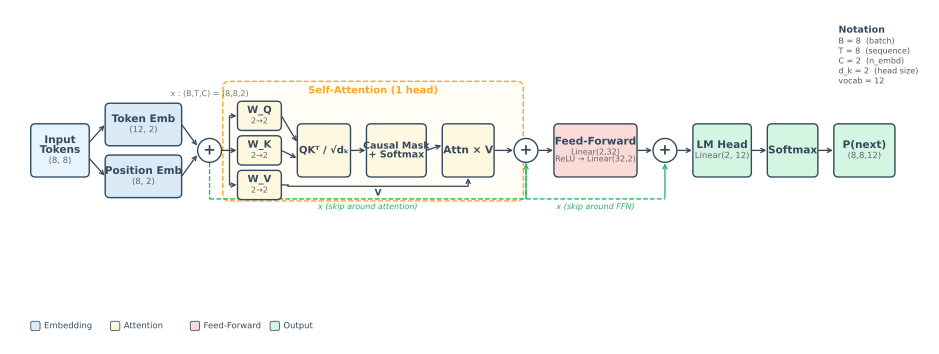
\includegraphics[width=\textwidth]{plus_last_even/plots/01_architecture_overview.png}
\caption{Architecture of the minimal transformer.}
\label{fig:architecture}
\end{figure}

\subsection{The Model Learns the Rule}

We first verify that training succeeds. Figure~\ref{fig:learning_curve} shows the training dynamics over 20{,}000 steps. Cross-entropy loss drops steeply in the first ${\sim}2{,}000$ steps as the model learns basic token frequencies, then continues to decrease more gradually as it acquires the conditional structure of the rule. More informatively, the rule error---the fraction of constrained positions (those immediately following \texttt{+}) where the model's top prediction is wrong---drops from approximately 90\% (chance level for a 12-token vocabulary) to near 0\%. The model has not merely memorized the training data; it has learned the underlying rule.

\begin{figure}[h]
\centering
\includegraphics[width=0.85\textwidth]{plus_last_even/plots/02_learning_curve.png}
\caption{Training loss and rule error over 20{,}000 steps.}
\label{fig:learning_curve}
\end{figure}

To confirm this, we examine both the training data and the model's own generations. Figure~\ref{fig:training_data} displays four sample training sequences as heatmaps, where green marks constrained positions with the correct label, red marks incorrect, and gray marks unconstrained (free) positions. All constrained positions are green, verifying the data generator. Figure~\ref{fig:generated} then compares sequences generated by the model before and after training. At initialization (step~0), predictions at constrained positions are essentially random---most cells are red. After training, nearly all constrained positions are green: the model reliably outputs the most recent even number after every \texttt{+}. The model works. The question now is \emph{how}.

\begin{figure}[h]
\centering
\includegraphics[width=0.85\textwidth]{plus_last_even/plots/03_training_data.png}
\caption{Sample training sequences. Green = correct at constrained positions.}
\label{fig:training_data}
\end{figure}

\begin{figure}[h]
\centering
\includegraphics[width=0.85\textwidth]{plus_last_even/plots/04_generated_sequences.png}
\caption{Model-generated sequences at initialization (top) vs.\ after training (bottom).}
\label{fig:generated}
\end{figure}

\subsection{The Embedding Space: How the Model Encodes Its Vocabulary}

The first stage of the transformer maps each input token and position to a 2D vector. Figure~\ref{fig:embeddings} reveals that the learned embedding layer has already done significant organizational work before any attention occurs. In the token embedding scatter plot (bottom-left), the six even numbers (0, 2, 4, 6, 8, 10) cluster together in one region of the plane, the five odd numbers (1, 3, 5, 7, 9) cluster separately, and the \texttt{+} operator sits far from both groups as an isolated outlier. The model has discovered, without supervision, that the categories relevant to the rule---even numbers, odd numbers, and the operator---should occupy geometrically distinct regions.

The position embeddings (bottom-center) form a near-linear vertical ladder, with $p_0$ at the bottom and $p_7$ at the top. This orderly arrangement allows the model to encode ``how far back'' a token is, which is essential for the ``most recent'' aspect of the rule. When token and position embeddings are summed (bottom-right), each token fans out into eight copies---one per position---shifted vertically by the position embedding. Crucially, even-number groups remain clearly separable from odd-number groups at every position, meaning the model can distinguish even from odd regardless of where in the context window a token appears.

\begin{figure}[h]
\centering
\includegraphics[width=\textwidth]{plus_last_even/plots/05_token_embeddings.png}
\caption{Learned embeddings. Bottom row: 2D scatter of token (left), position (center), and combined (right) embeddings.}
\label{fig:embeddings}
\end{figure}

This structure does not exist at initialization. Movie~1 shows the embedding space at every checkpoint across training. At step~0, all points are randomly scattered. Within the first few thousand steps, the \texttt{+} token rapidly migrates away from the number tokens. The even/odd split solidifies between steps 5{,}000 and 10{,}000, and the position ladder organizes gradually throughout training. The embedding geometry is not hand-designed; it is the structure that gradient descent discovers in service of the rule.

\subsection{The Output Landscape: Where Representations Need to Land}

Before examining the attention mechanism, it is useful to understand the \emph{destination}: given a 2D point after all processing, what does the model predict? The LM head is a linear map followed by softmax, so it partitions the 2D plane into decision regions---one per output token---separated by linear boundaries. Figure~\ref{fig:output_landscape} makes this partition explicit. Each subplot shows the probability that the model assigns to one particular output token, evaluated at every point on the plane (yellow = high, purple $\approx 0$), with all 96 token+position embeddings annotated at their starting coordinates.

Several observations are immediately apparent. First, each even number occupies its own distinct high-probability stripe. The stripe for token~0 lies in one part of the plane, the stripe for token~2 in another, and so on for 4, 6, 8, and 10---they tile the region of the plane where \texttt{+} embeddings will land after attention processing. Second, the high-probability region for \texttt{+} as the next token spans the broad area where number embeddings reside, consistent with the 30\% base rate of \texttt{+} in the training data. Third, odd numbers have their own probability regions, but these are less sharply defined because odd-number predictions are never required by the rule---they are only predicted at unconstrained positions.

The critical implication is this: for the model to correctly output, say, token~8 after a \texttt{+}, the \texttt{+} position's representation must be \emph{moved}---by attention and the residual connection---from its starting location in the \texttt{+} cluster to the specific stripe where $P(\text{next}=8)$ is high. The remaining figures will show exactly how the model accomplishes this movement.

\begin{figure}[t]
\centering
\includegraphics[width=\textwidth]{plus_last_even/plots/07_output_probs_embed.png}
\caption{Output probability landscape. Each subplot shows $P(\text{next} = \text{token})$ over the 2D plane, with all token+position embeddings annotated.}
\label{fig:output_landscape}
\end{figure}

The output landscape and the embedding positions co-evolve during training (Movie~2). At initialization, the probability landscape is nearly uniform---no decision boundaries exist. As the model first learns token frequencies, broad regions form. These sharpen progressively into the final configuration where each even number has a well-defined, non-overlapping high-probability region in exactly the part of the plane that the attention mechanism will target.

\subsection{The Attention Mechanism: Query, Key, and Value Projections}

The bridge between the starting embeddings and the output landscape is self-attention. The model applies three learned $2 \times 2$ linear transformations---$W_Q$, $W_K$, $W_V$---to every token+position embedding, producing query, key, and value vectors respectively. Figure~\ref{fig:qkv} shows these transformations and their effect. The original embedding space (top-left) is transformed into three distinct spaces: the query space (blue), the key space (red), and the value space (green). Each transformation stretches, rotates, and rearranges the points differently, reflecting the different roles these vectors play.

The query and key transformations jointly determine \emph{who attends to whom}: the dot product between a query and a key controls the attention weight. The value transformation determines \emph{what information gets routed}: the attention-weighted sum of value vectors is what actually gets added to the residual stream. These three spaces must be coordinated---the Q/K geometry must select the right positions, and the V geometry must carry the right information to those positions. Movie~3 shows that early in training, all three projections produce nearly identical spaces, but they progressively specialize as the model learns to implement the rule.

\begin{figure}[h]
\centering
\includegraphics[width=\textwidth]{plus_last_even/plots/08_qkv_transforms.png}
\caption{QKV projections. Top: weight matrices as heatmaps. Bottom: all 96 token+position embeddings after each projection.}
\label{fig:qkv}
\end{figure}

\subsection{Who Attends to Whom: The Query--Key Geometry}

The question at the heart of the plus-last-even rule is: when the model encounters a \texttt{+}, how does it know to look back and find the most recent even number? The answer lies in the geometry of the query--key space. Figure~\ref{fig:qk_space} plots all 96 query vectors (blue) and all 96 key vectors (red) on common axes, so we can directly read off the attention pattern from the spatial relationships.

The \texttt{+} queries form a tight, isolated cluster, well-separated from all number queries. More importantly, the direction from the origin to this \texttt{+} cluster is geometrically aligned with the keys of even-number tokens---that is, the dot product between a \texttt{+} query and an even-number key is large, producing strong attention. In contrast, the dot product between a \texttt{+} query and an odd-number key is small, producing weak attention. This is the geometric encoding of the rule's core requirement: \texttt{+} should attend to even numbers and ignore odd numbers.

But the rule demands more than just ``attend to even numbers''---it requires attending to the \emph{most recent} one. This is encoded in the positional spread of each token's keys. Within the key cluster for any given even number, keys at later positions (closer to the query) are arranged so that they have slightly higher dot products with the \texttt{+} query than keys at earlier positions. After softmax normalization, this bias means the most recent even number receives the highest attention weight. The position embeddings' orderly ladder structure (Figure~\ref{fig:embeddings}) feeds directly into this: position information is preserved through the key projection and manifests as a recency gradient in the Q/K dot products.

\begin{figure}[h]
\centering
\includegraphics[width=0.85\textwidth]{plus_last_even/plots/09_qk_space.png}
\caption{Joint query--key space. Blue: queries. Red: keys. Labels show token and position.}
\label{fig:qk_space}
\end{figure}

Movie~4 reveals how this structure develops over the course of training. At initialization, queries and keys are intermingled with no meaningful separation. Over the first several thousand steps, the \texttt{+} queries begin migrating away from the number queries. Simultaneously, even-number keys separate from odd-number keys along the axis that aligns with the \texttt{+} query direction. By the end of training, the geometry has converged to the configuration described above: a clear \texttt{+} query cluster aligned with even-number keys and orthogonal to odd-number keys.

To make the attention pattern even more concrete, Figure~\ref{fig:qk_focus} isolates a single query---\texttt{+} at position~5---and colors the entire Q/K plane by its dot product with that query. The resulting gradient shows high values (green) concentrated at the locations of even-number keys at positions 0--4, and low values (white) at odd-number key locations. Keys at positions $\geq 5$ are irrelevant due to the causal mask. This is the retrieval mechanism laid bare: the \texttt{+} query acts as a selective filter that picks out even-number keys from the past context, with recency biasing the selection toward the most recent one.

\begin{figure}[h]
\centering
\includegraphics[width=0.85\textwidth]{plus_last_even/plots/10_qk_space_focus.png}
\caption{Dot-product gradient for the query \texttt{+} at position~5. Green = high attention.}
\label{fig:qk_focus}
\end{figure}

The full $96 \times 96$ attention score matrix (Figure~\ref{fig:attention_matrix}) confirms that this pattern generalizes across all token--position combinations. The matrix is organized as a $12 \times 12$ grid of blocks, where each block represents one query-token versus one key-token, with the 8 positions arranged within each block. The bottom row---corresponding to \texttt{+} as the query token---is the most informative: even-number key columns (0, 2, 4, 6, 8, 10) show warm colors (high attention scores), while odd-number key columns show cool colors (low scores). The \texttt{+} operator attends selectively and strongly to even numbers, regardless of position. Movie~5 shows this row sharpening from a diffuse pattern at initialization to the clean even/odd dichotomy observed in the final model.

\begin{figure}[h]
\centering
\includegraphics[width=\textwidth]{plus_last_even/plots/11_qk_full_heatmap.png}
\caption{Full $96 \times 96$ attention score matrix, organized as a $12 \times 12$ grid of token--token blocks.}
\label{fig:attention_matrix}
\end{figure}

\subsection{What Gets Retrieved: The Value Space}

The Q/K geometry determines \emph{where} the model looks; the value transformation determines \emph{what information} it extracts. Figure~\ref{fig:value_landscape} overlays the value-transformed vectors ($W_V$ applied to each token+position embedding) on the same probability heatmaps from Figure~\ref{fig:output_landscape}. The key observation is that the value vectors for each even number are positioned so that, after being selected by attention and summed, the resulting vector lands in the high-probability region for that even number in the output landscape. The model has learned a value transformation that is \emph{coordinated} with the LM head's decision boundaries: $V$ carries information in a form that the output layer can directly decode.

\begin{figure}[h]
\centering
\includegraphics[width=\textwidth]{plus_last_even/plots/12_probability_heatmap_with_values.png}
\caption{Output probability landscape with value-transformed vectors overlaid (cf.\ Figure~\ref{fig:output_landscape}, which shows raw embeddings).}
\label{fig:value_landscape}
\end{figure}

\subsection{Tracing a Sequence Through the Pipeline}

The preceding analysis characterized the model's learned parameters in the abstract---all 96 possible token+position combinations. We now ground this analysis by tracing a single concrete sequence, \texttt{10 + 10 6 + 6 4 8}, through the complete inference pipeline and verifying that each step works as predicted.

\paragraph{Embedding.} Figure~\ref{fig:seq_embed} shows where each token in this specific sequence lands in embedding space. The \texttt{+} tokens at positions~1 and~4 are located far from the number tokens, exactly as the global structure predicts. The number tokens fan out according to their position offsets, with even numbers (10, 6, 4, 8) and odd numbers in their respective global clusters. This sequence contains two constrained positions: position~2 (which follows the first \texttt{+}, with the last even being~10) and position~5 (which follows the second \texttt{+}, with the last even being~6).

\begin{figure}[h]
\centering
\includegraphics[width=\textwidth]{plus_last_even/plots/13_sequence_embeddings.png}
\caption{Embeddings for the demo sequence \texttt{10 + 10 6 + 6 4 8}, shown as heatmaps (top) and 2D scatter (bottom).}
\label{fig:seq_embed}
\end{figure}

\paragraph{Attention.} Figure~\ref{fig:seq_attention} displays the full attention computation for this sequence. The Q/K scatter (panel~3) shows the sequence's query and key vectors against the global backdrop---the \texttt{+} queries at positions~1 and~4 are visibly isolated in the region that aligns with even-number keys. The raw attention scores (panel~4, before softmax) show high values where \texttt{+} queries meet keys from positions containing even numbers, and the final attention matrix (panel~5, after softmax) confirms the expected pattern. At position~2 (the token after the first \texttt{+}), the model attends overwhelmingly to position~0, which contains 10---the most recent even number before that \texttt{+}. At position~5 (the token after the second \texttt{+}), the model attends most strongly to position~3, which contains 6---the most recent even number before the second \texttt{+}. The retrieval mechanism identified in the global analysis (Figures~\ref{fig:qk_space}--\ref{fig:attention_matrix}) is operating exactly as predicted on real inputs.

\begin{figure}[h]
\centering
\includegraphics[width=\textwidth]{plus_last_even/plots/14_qk_attention.png}
\caption{Attention computation for the demo sequence. Panels: Q heatmap, K heatmap, Q/K scatter, raw scores, attention weights.}
\label{fig:seq_attention}
\end{figure}

\paragraph{Value routing.} Figure~\ref{fig:seq_value} completes the attention story by showing what information is actually extracted. The attention-weighted sum of value vectors at each position (panel~3) represents the ``message'' that attention delivers to the residual stream. At the two constrained positions, the attention output is dominated by the value vector of the attended even number---token~10 and token~6, respectively. The attention-output scatter (panel~5) shows where these messages land in 2D space: they point toward the regions where the output landscape (Figure~\ref{fig:output_landscape}) assigns high probability to the correct answer.

\begin{figure}[h]
\centering
\includegraphics[width=\textwidth]{plus_last_even/plots/15_value_output.png}
\caption{Value pathway for the demo sequence. Panels: attention weights, V vectors, attention output, V scatter, output scatter.}
\label{fig:seq_value}
\end{figure}

\paragraph{Residual stream.} The attention output does not replace the input---it is \emph{added} to it via the residual connection. Figure~\ref{fig:residuals} visualizes this addition. The bottom row shows, in 2D, the input embedding at each position, the attention output, and arrows illustrating how the residual sum shifts each position's representation. The critical observation is in the arrow plot (panel~c): at the two \texttt{+} positions, the arrows are large and point decisively toward the region of the plane associated with the correct even number. The attention mechanism is literally \emph{moving} the \texttt{+} representation from its starting location in the operator cluster toward the decision region for the correct output token. At unconstrained positions---where the model does not need to implement the rule---the arrows are smaller and less directed, leaving those representations relatively undisturbed.

\begin{figure}[h]
\centering
\includegraphics[width=\textwidth]{plus_last_even/plots/16_residuals.png}
\caption{Residual stream for the demo sequence. Bottom row: embeddings~(a), attention output arrows~(b), residual shift arrows~(c), and final representations~(d).}
\label{fig:residuals}
\end{figure}

\paragraph{Output verification.} Finally, Figure~\ref{fig:final_grid} provides the empirical proof that the full pipeline works. Each subplot overlays the post-residual positions on the output probability heatmaps from Figure~\ref{fig:output_landscape}. At every constrained position, the final representation---after attention has routed the correct value and the residual connection has shifted the state---sits squarely inside the high-probability region for the correct even number. The \texttt{+} at position~1 has been moved into the region where $P(\text{next}=10)$ is maximal. The \texttt{+} at position~4 has been moved into the region where $P(\text{next}=6)$ is maximal. The geometry has executed the algorithm: detect \texttt{+}, retrieve the most recent even number, route its value through the residual, and land in the correct output region.

\begin{figure}[h]
\centering
\includegraphics[width=\textwidth]{plus_last_even/plots/17_final_on_output_grid.png}
\caption{Final post-residual representations overlaid on the output probability landscape. Each \texttt{+} position lands in the high-probability region for the correct even number.}
\label{fig:final_grid}
\end{figure}

%----------------------------------------------------------------------
\section{Geometry as Algorithm: Summary}

For the plus-last-even rule, the model's behavior decomposes into a five-step algorithm. Each step corresponds to a specific geometric structure visible in the preceding figures.

\begin{enumerate}
    \item \textbf{Encode.} Map each (token, position) pair to a 2D point: $\mathbf{x}_i = E_{t_i} + P_i$. The embedding scatter plots (Figure~\ref{fig:embeddings}) show this mapping, with even numbers, odd numbers, and \texttt{+} occupying distinct regions.

    \item \textbf{Detect the operator.} The query projection $W_Q$ maps the \texttt{+} embedding to a query vector that is geometrically distinct from number queries. The Q/K embedding space (Figure~\ref{fig:qk_space}) shows \texttt{+} queries forming a separate cluster.

    \item \textbf{Retrieve the last even number.} The dot product between the \texttt{+} query and all keys yields high attention weight for even-number keys, with recency encoded in the positional component of the key layout. The focused-query analysis (Figure~\ref{fig:qk_focus}) and full attention matrix (Figure~\ref{fig:attention_matrix}) make this retrieval pattern explicit.

    \item \textbf{Route value through residual.} Attention selects the value vector at the most recent even-number position; the residual connection adds it to the current state. The residual stream visualization (Figure~\ref{fig:residuals}) shows the \texttt{+} position's representation being displaced toward the correct even number's region.

    \item \textbf{Output.} The LM head partitions $\mathbb{R}^2$ into decision regions, one per token. The post-residual state lands in the region corresponding to the correct even number, and softmax produces the prediction. The output probability heatmaps (Figure~\ref{fig:output_landscape}) and the final-state overlay (Figure~\ref{fig:final_grid}) confirm this.
\end{enumerate}

The geometry \emph{is} the algorithm. There is no separate procedure hidden in the weights; the 2D arrangement of points and decision boundaries is itself the step-by-step computation the model executes.

%----------------------------------------------------------------------
\section{Discussion}

\paragraph{Why two dimensions?} Constraining $n_{\mathrm{embd}} = 2$ and $d_k = 2$ sacrifices expressiveness for complete interpretability. The model must implement the rule in a low-dimensional space, which forces it to discover a compact solution. Every state and every boundary is directly visible without projection artifacts. For many procedural rules (copy-modulo, successor, plus-last-even), two dimensions suffice for high accuracy. For harder tasks, the framework could be extended to $n_{\mathrm{embd}} = 4$ or higher, using paired 2D projections to retain partial interpretability.

\paragraph{Limitations.} (1)~The rules are synthetic and the vocabulary is small; transfer to natural-language tasks or more complex reasoning remains an open question. (2)~We use a single head and a single block; deeper or wider models would require dimensionality reduction or other tools. (3)~Some rules may require more than two dimensions to learn efficiently; we have not systematically tested the minimal sufficient dimensionality. (4)~The algorithmic reading is a qualitative interpretation of the geometry; we do not provide a formal proof that the model ``implements'' this algorithm, though the figures constitute strong evidence.

\paragraph{Future directions.} Natural extensions include automating the geometry-to-algorithm description (e.g., by programmatically summarizing attention patterns and decision boundaries), comparing the learned geometry across different rules to identify common algorithmic motifs, and testing whether targeted interventions in embedding space (e.g., ablating a direction) produce the predicted behavioral change---thereby establishing that the geometry is causally related to the algorithm.

%----------------------------------------------------------------------
\section{Movies}

The following animations show the evolution of the model's learned geometry over the course of training (one frame per checkpoint, 200 frames total). These are available as GIF/MP4 files in \texttt{plus\_last\_even/plots/learning\_dynamics/}.

\begin{table}[h]
\centering
\caption{Training-dynamics animations (supplementary).}
\label{tab:movies}
\begin{tabular}{lp{9cm}}
\toprule
Movie & Description \\
\midrule
Movie~1 & Evolution of token, position, and combined embedding scatter plots. The \texttt{+} token separates from numbers first; the even/odd split solidifies by step 5{,}000--10{,}000. \\
Movie~2 & Co-evolution of the LM head's output probability landscape and embedding positions. Decision boundaries sharpen progressively from a uniform initialization. \\
Movie~3 & Specialization of the Q, K, and V subspaces. All three projections are initially identical and develop distinct geometry as training progresses. \\
Movie~4 & Separation of query and key subspaces. \texttt{+} queries migrate away from number queries; even-number keys align with the \texttt{+} query direction. \\
Movie~5 & Evolution of the full attention matrix alongside the Q/K scatter. The \texttt{+}-row entries concentrate on even-number columns over training. \\
\bottomrule
\end{tabular}
\end{table}

%----------------------------------------------------------------------

\begin{thebibliography}{9}

\bibitem{bhattamishra2020}
Bhattamishra, S., Ahuja, K., \& Goyal, N. (2020).
On the computational power of transformers and its implications in sequence modeling.
\emph{CoRR}, abs/2006.09286.

\bibitem{clark2019}
Clark, K., Khandelwal, U., Levy, O., \& Manning, C.\,D. (2019).
What does BERT look at? An analysis of BERT's attention.
\emph{ACL Workshop on BlackboxNLP}.

\bibitem{hewitt2019}
Hewitt, J. \& Liang, P. (2019).
Designing and interpreting probes with control tasks.
\emph{EMNLP}.

\bibitem{mikolov2013}
Mikolov, T., Sutskever, I., Chen, K., Corrado, G.\,S., \& Dean, J. (2013).
Distributed representations of words and phrases and their compositionality.
\emph{NeurIPS}.

\bibitem{olsson2022}
Olsson, C., Elhage, N., Nanda, N., et al. (2022).
In-context learning and induction heads.
\emph{Transformer Circuits Thread}.

\bibitem{vandermaaten2008}
van der Maaten, L. \& Hinton, G. (2008).
Visualizing data using t-SNE.
\emph{JMLR}, 9, 2579--2605.

\bibitem{vig2019}
Vig, J. (2019).
A multiscale visualization of attention in the transformer model.
\emph{ACL System Demonstrations}.

\bibitem{wang2022}
Wang, K., Variengien, A., Conmy, A., Shlegeris, B., \& Steinhardt, J. (2022).
Interpretability in the wild: A circuit for indirect object identification in GPT-2 small.
\emph{NeurIPS}.

\bibitem{weiss2018}
Weiss, G., Goldberg, Y., \& Yahav, E. (2018).
On the practical computational power of finite precision RNNs for language recognition.
\emph{ACL}.

\end{thebibliography}

\end{document}
